\documentclass[border = 0.2cm]{standalone}

\usepackage{tikz}
\usepackage{pgf}
\usetikzlibrary{snakes, mindmap, trees}

\tikzstyle{level 1} = [sibling angle = 120]
\tikzstyle{level 2} = [sibling angle = 60]
\tikzstyle{level 3} = [sibling angle = 30]
\tikzstyle{every node} = [fill]
\tikzstyle{edge from parent} = [snake = expanding waves, segment length = 1mm, segment angle = 10, draw]

\begin{document}
    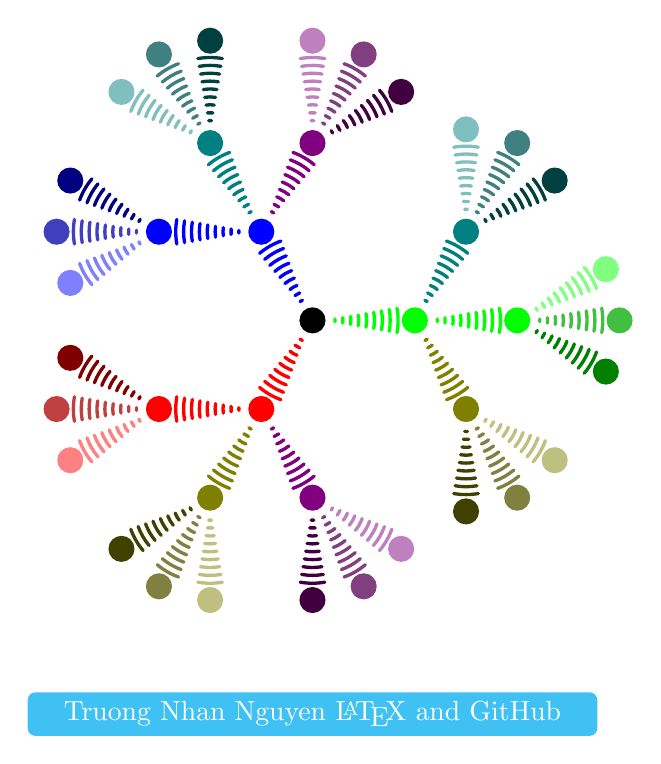
\begin{tikzpicture}[grow cyclic, shape = circle, very thick, level distance = 13mm, cap = round]
        \node {} child [color = \A] foreach \A in {red, green, blue}
        {
            node {} child [color = \A!50!\B] foreach \B in {red, green, blue}
            {
                node {} child [color = \A!50!\B!50!\C] foreach \C in {black, gray, white}
                {
                    node {}
                }
            }
        };

        \begin{scope}[yshift = -5cm]
            \node [fill = cyan!75, text = white, rectangle, text width = 7cm,
                    rounded corners = 0.1cm, text centered
            ]
            {Truong Nhan Nguyen \LaTeX{} and GitHub};
        \end{scope}
    \end{tikzpicture}
\end{document}